\chapter{The Software} \label{chap:software}

Two main types of software are required for the operation of this kind of aircraft. The flight controller runs on the on-board computer and is responsible for controlling the flight itself, and a ground station software, responsible for higher level commands and telemetry.
This chapters details these software used in the project.

\begin{figure}[h]
  \centering
  \begin{subfigure}{.5\textwidth}
    \centering
    
\includegraphics[width=\linewidth]{figs/px4.png}
  \end{subfigure}%
  \begin{subfigure}{.5\textwidth}
    \centering
    
\includegraphics[width=\linewidth]{figs/ardupilot.png}

  \end{subfigure}
  \caption{PX4 and Ardupilot.}
  \label{fig:softwares}
\end{figure}


\section{Flight Controller}
The flight controller software runs on the on-board computer, and is responsible for controlling the attitude, altitude, and position of the aircraft.
%
In order to achieve this, most flight controller boards come with internal sensors (accelerometer, gyroscope, magnetometer, barometer) and external ones (airspeed, magnetometer, GPS). 
%
The acquired data is used to estimate attitude and position, which is then corrected by the control loops.

The possible choices of flight controller software were ArduPilot and PX4.
%
Ardupilot is a community-drive software started by DYIDrones in 2009\cite{diydrones}.
%
It is GPL licensed, which means all changes made and commercialized must be open-sourced\cite{gplv3}.
%
ArduPilot is a mature software, with a large community of users and testers.
%
%https://github.com/PX4/Firmware/commits/master?after=3e0b8b7016556224aedb54f51d769d3288f0920e+24770

PX4 was also developed since 2008[\cite{waybackmachine}, mostly by the Computer Vision and Geometry Lab of ETH Zurich (Swiss Federal Institute of Technology)\cite{computervision} and the Autonomous Systems Lab\cite{autonomouslab} under a more permissive BSD 3-clause license\cite{bsd}.
%
For a while both projects worked closely, the Pixhawk Flight Controller board is a result of this interaction.
%
Both also joined Dronecode\cite{dronecode}, a Linux Foundation\cite{linuxfoundation} initiative started in 2004 as an attempt to grow the UAV ecosystem and reach larger companies.
%

Dronecode however, evolved into, according to the Ardupilot Dev Team, a flawed model.
%
It was required for all projects to hand over all domains, accounts, and trademarks to their control.
%
The projects are also directed by the so-called "Platinum Members", which means the development would not be in control of the community anymore.
%
By September 9, 2016, a letter was released stating that Ardupilot was leaving Dronecode, and explaining why\cite{letter}.

The Ardupilot code was chosen for this project due to their larger openness and community.

Ardupilot is split into four main sub-projects:
\begin{itemize}
\item ArduCopter is a Flight controller for helicopters and Multirotors.
\item ArduPlane is Focused on fixed wing aircraft, but now includes some of the ArduCopter control loops for VTOL capabilities.
\item ArduHover is focused on land vehicles and aquatic surface vehicles.
\item ArduSub is a controller for submersible vehicles.
\end{itemize}

While each of them has different features, they share most of the core ArduPilot code.

Arduplane provides all required controllers for features such as automatic vertical take off and landing, fixed-wing flight, waypoint navigation, inverted flight, stall prevention, geo-fencing, and terrain following, more than enough for performing the tasks proposed in this project.

\section{Software Architecture}

The ArduPilot codebase is split into four main projects, they all do however have the common base, an thus, a similar architecture. On Figure \ref{fig:highlevel} the high level architecture is shown, presenting an overview of the main interactions between hardware and software components, from the ground station, to the communication protocol, to the low-level sensors.

\begin{figure}[h]
\centering
  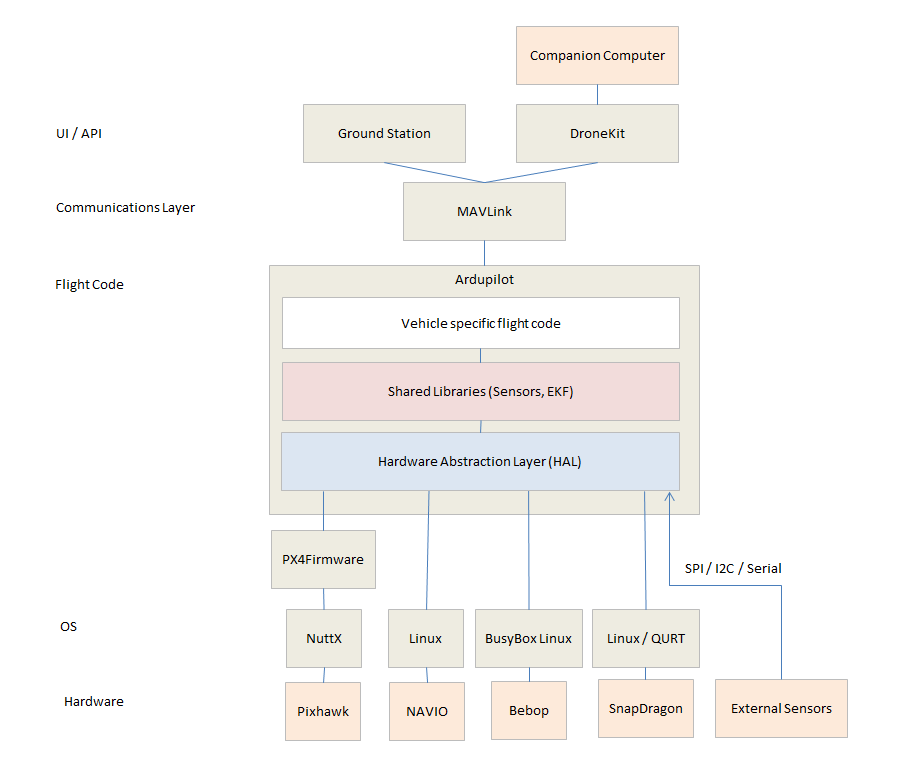
\includegraphics[width=0.95\linewidth]{figs/highlevelarch.png}
  \caption{ArduPilot high-level software architecture. Source: ArduPilot.org}
  \label{fig:highlevel}
\end{figure}

A more detailed diagram, on Figure \ref{fig:lowlevel} details the interactions on a source-code file level. Additional information is available at the project's website, as well as the source code\cite{ardupilotcode}.


\begin{figure}[h]
\centering
  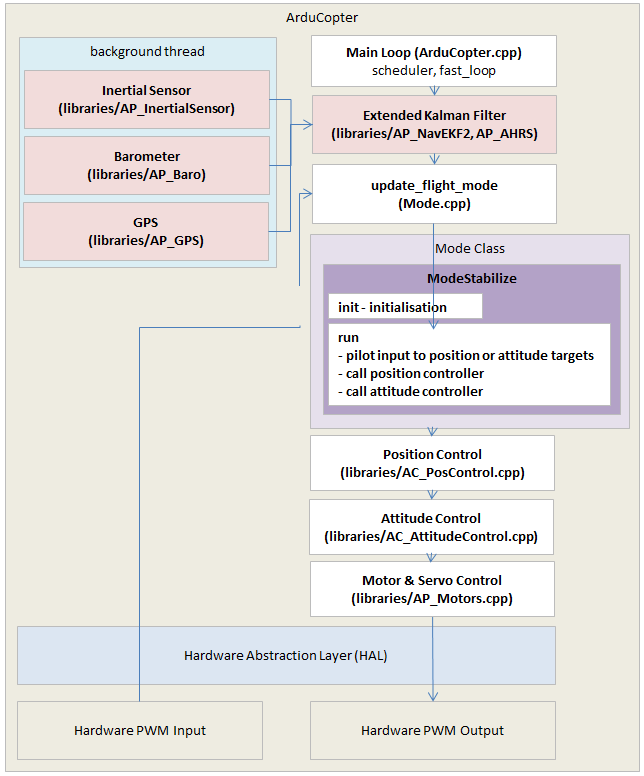
\includegraphics[width=0.8\linewidth]{figs/copter-architecture.png}
  \caption{ArduPilot high-level software architecture. Source: ArduPilot.org}
  \label{fig:lowlevel}
\end{figure}


\section{Ground Station Software}

For ground station software, there are two major players, ardupilot's own MissionPlanner, and KDE's QGroundControl.

MissionPlanner is developed in C\# and is generally more up-to-date with Arduplane.
%
It does however have performance issues and is not compatible with Linux.
%

QGroundControl is a C++ and Qt based software, boasting a high performance and well-finished interface, as well as compatibility with windows, Linux, OS-X and Android. But as it attempts to support both ArduPilot and PX4, eventually the Ardupilot support is not up to date.
%

Both are able to do the basic aircraft setup, change modes, and setup parameters via wired or wireless connections. As both have upsides and downsides, both were used in the project. QGroundControl was used whenever possible, and, when it couldn't perform something, MissionPlanner was used.

Additionally, Mavproxy\cite{mavproxy} and APM Planner 2\cite{apm2} were used to view logs and export them to Google Earth

\begin{figure}[h]
  \centering
  \begin{subfigure}{.8\textwidth}
    \centering
    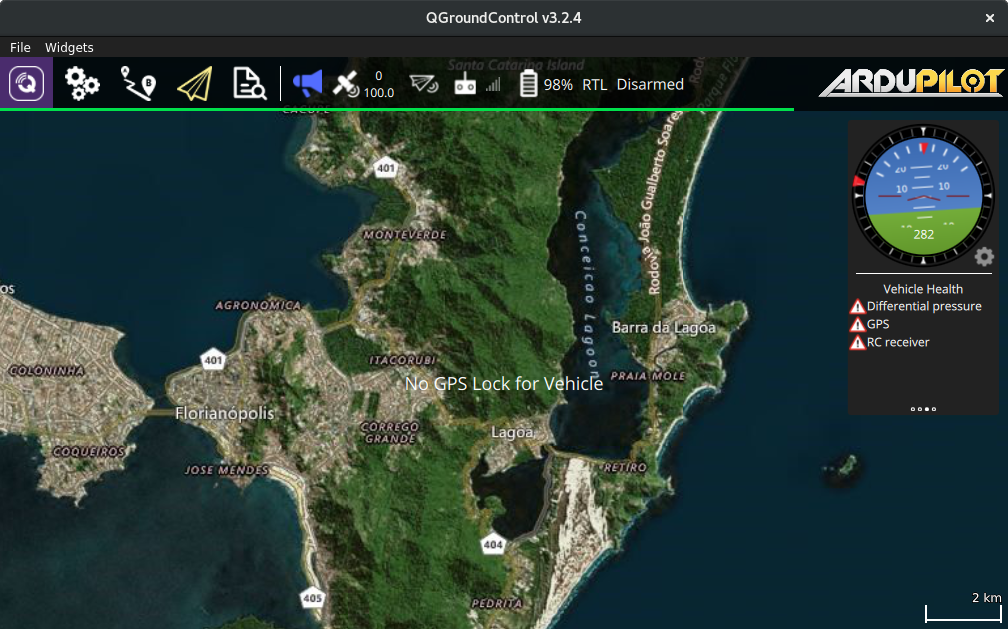
\includegraphics[width=\linewidth]{figs/qgc.png}
  \end{subfigure}%

  \begin{subfigure}{.8\textwidth}
    \centering
    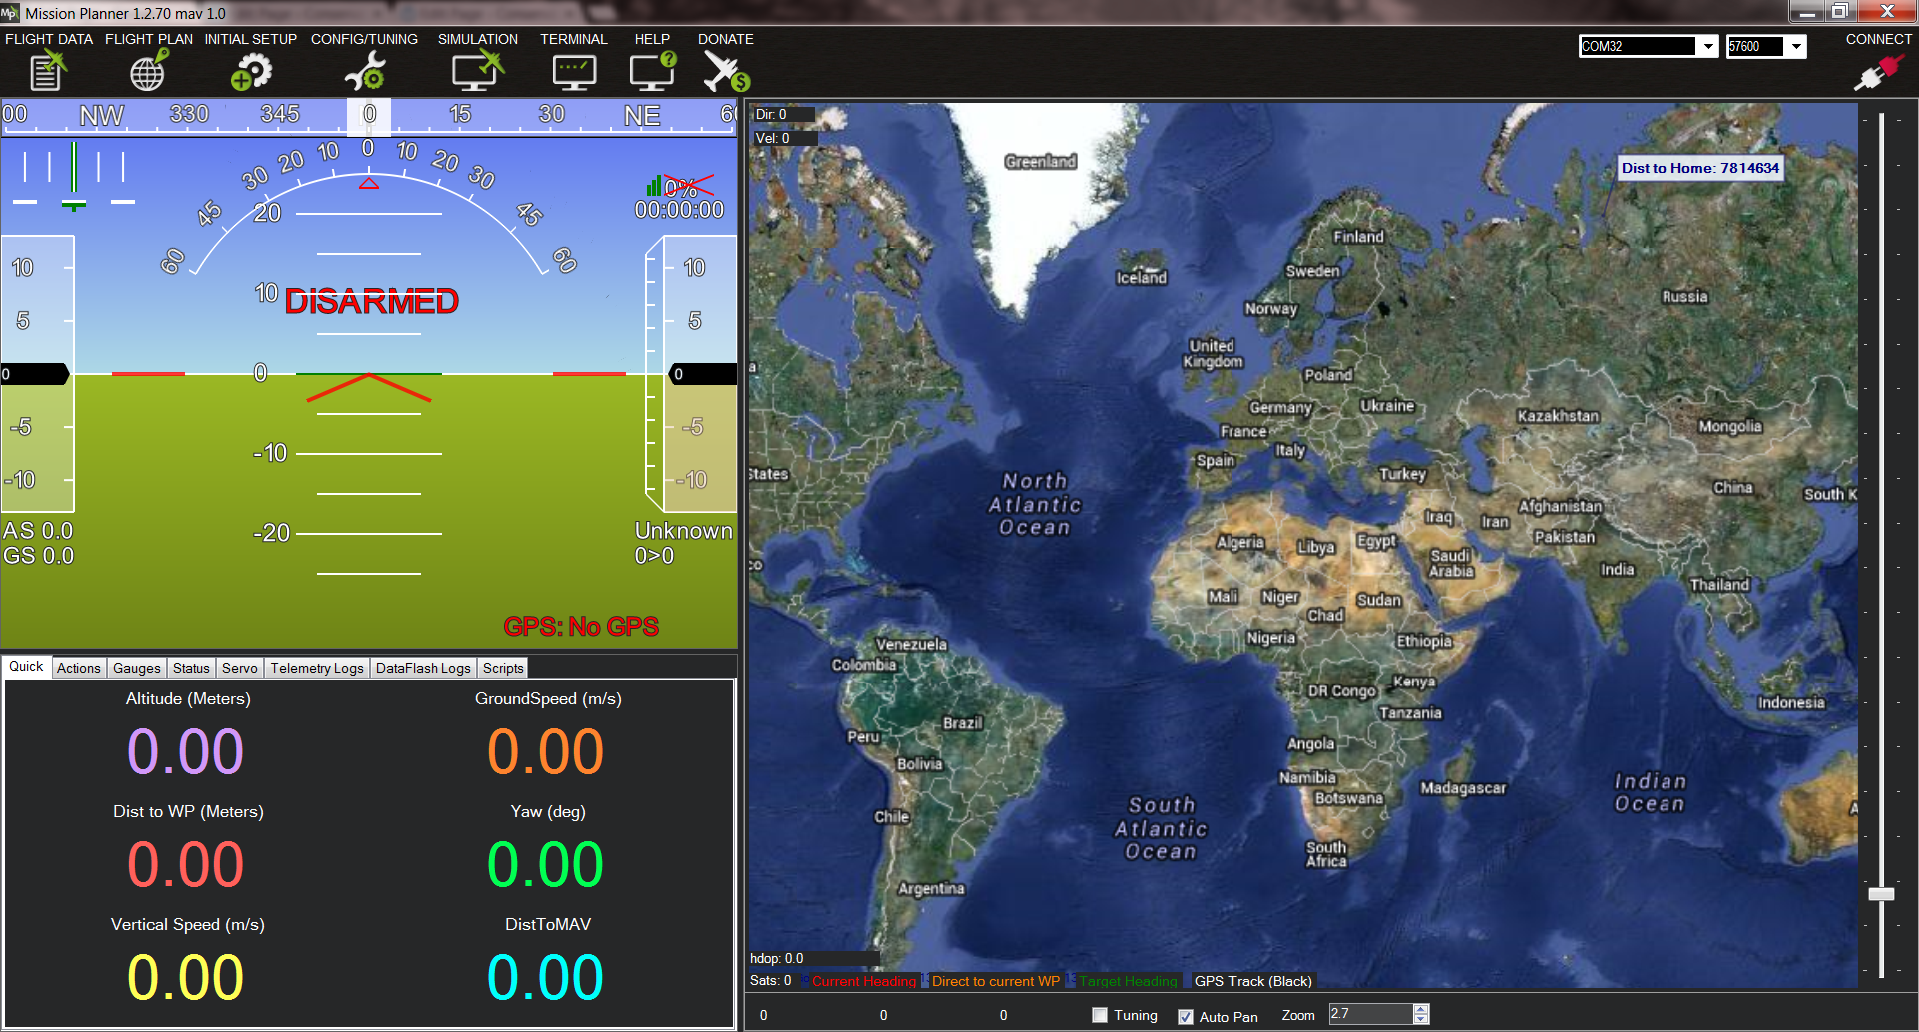
\includegraphics[width=\linewidth]{figs/missionplanner.png}

  \end{subfigure}
  \caption{QGroundControl and MissionPlanner.}
  \label{fig:groudstations}
\end{figure}